%%%%%%%%%%%%%%%%%%%%%%%%%%%%%%%%%%%%%%%%%%%%%%%%%%%%%%%%%%%%%%%%%%%%%%%%%%%%%%%%
% Frontiers Supplementary Material file prepared from the original appendix source.
%%%%%%%%%%%%%%%%%%%%%%%%%%%%%%%%%%%%%%%%%%%%%%%%%%%%%%%%%%%%%%%%%%%%%%%%%%%%%%%%

\documentclass[utf8]{frontiers_suppmat}

\usepackage{url,hyperref,microtype}
\usepackage{booktabs,longtable,tabularx,threeparttable}
\usepackage{rotating,pdflscape,adjustbox,makecell}
\usepackage{array}
\usepackage{caption}
\usepackage[usenames,dvipsnames]{xcolor}

\newcommand{\offroi}[1]{\textcolor{black}{#1}}
\newcommand{\onroi}[1]{\textcolor{black}{#1}}
\newcommand{\commonroi}[1]{\textcolor{purple}{#1}}

\begin{document}
\onecolumn
\firstpage{1}

\title[Supplementary Material]{{\helveticaitalic{Supplementary Material}}}
\maketitle

\setcounter{figure}{0}
\setcounter{table}{0}
\renewcommand{\thefigure}{S\arabic{figure}}
\renewcommand{\thetable}{S\arabic{table}}


%##########################################################################################
\section{Behaviour Information}
Behaviour trial flow and quality-control summary. Each subject/session/run has a total.

\begin{figure} [h]
    \centering
    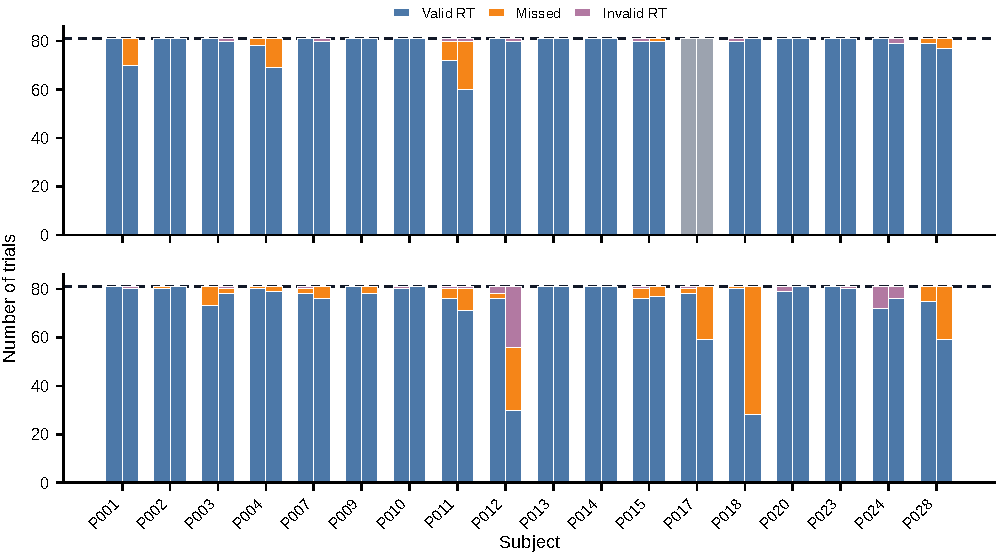
\includegraphics[width=\linewidth]{supplementary_figures/Sup_Figure25.pdf}
    \caption{Reaction-time quality-control summary. Stacked bars show trial information for each subject, medication session, and run; top and bottom panels show OFF and ON medication, respectively. Within each subject, the left and right bars correspond to runs 1 and 2. Each run contained 90 trials, including 9 catch trials not shown here and 81 go trials, marked by the dashed horizontal line. Valid RT trials were go trials with finite positive \(1/\mathrm{RT}\) values; missed trials were go trials flagged as no-squeeze trials \(1/\mathrm{RT}\). The gray color shows a subject for whom we don't have fMRI data.}
    \label{fig:RT_information}
\end{figure}


Reaction times were modestly faster in the ON-medication condition than in the OFF-medication condition. This pattern was visible both in the trial-wise RT distributions, where the ON distribution was slightly shifted toward shorter latencies, and in the subject-paired means, where most participants showed lower mean RT ON medication. The paired subject-level test showed a mean ON-OFF difference of $-13.6$ ms, $95\%$ CI $[-27.5, 0.3]$, $t(16) = -2.08$, p = $.054$, indicating a small medication-related speeding effect that approached but did not reach conventional significance. By comparison, temporal effects within the task were limited: RT was only slightly slower in run $2$ than run $1$, block position showed a mild increase in RT consistent with weak fatigue or time-on-task effects, and trial position within blocks showed no clear monotonic practice or drift pattern. Overall, the behavioural results suggest a small medication-associated reduction in RT, with practice, fatigue, and within-task drift contributing only modestly to RT variation. 

\begin{figure}[h]
    \centering
    \begin{minipage}[h]{0.4\textwidth}
        \centering
        \textbf{A}\\[-0.1em]
        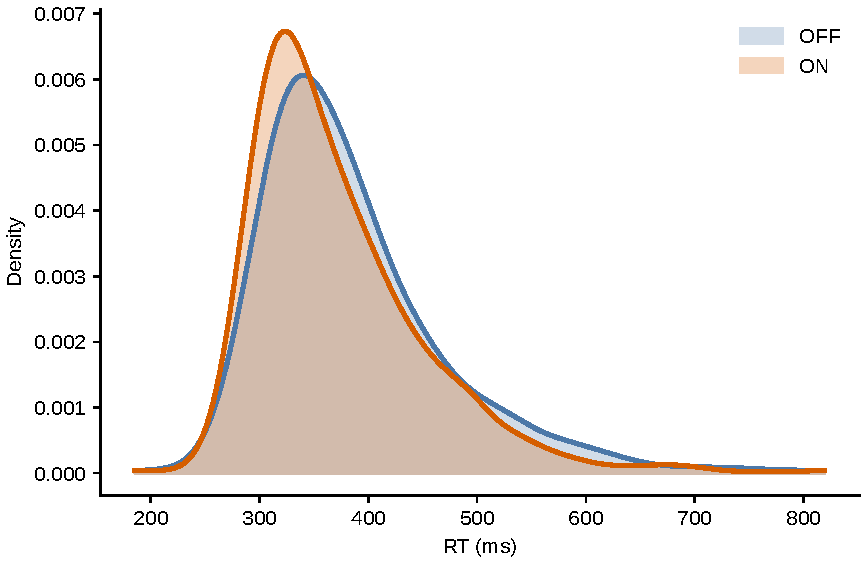
\includegraphics[height=0.9\textwidth,keepaspectratio]{supplementary_figures/Sup_Figure26.pdf}
    \end{minipage}
    \hfill
    \begin{minipage}[h]{0.5\textwidth}
        \centering
        \textbf{B}\\[-0.1em]
        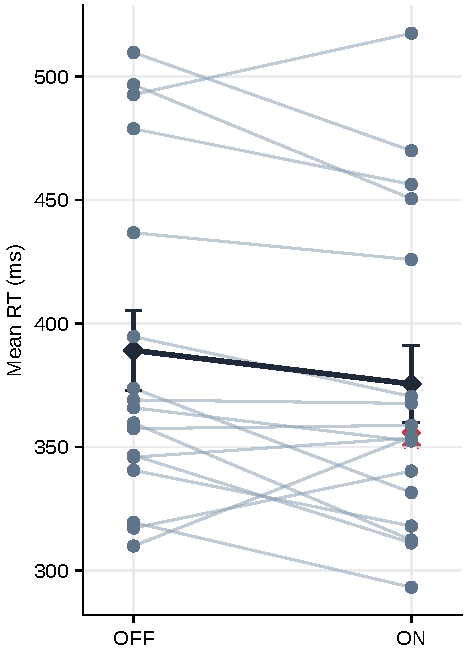
\includegraphics[height=0.7\textwidth,keepaspectratio]{supplementary_figures/Sup_Figure27.pdf}
    \end{minipage}

    \vspace{2em}

    \begin{minipage}[t]{\textwidth}
        \centering
        \textbf{C}\\[-0.1em]
        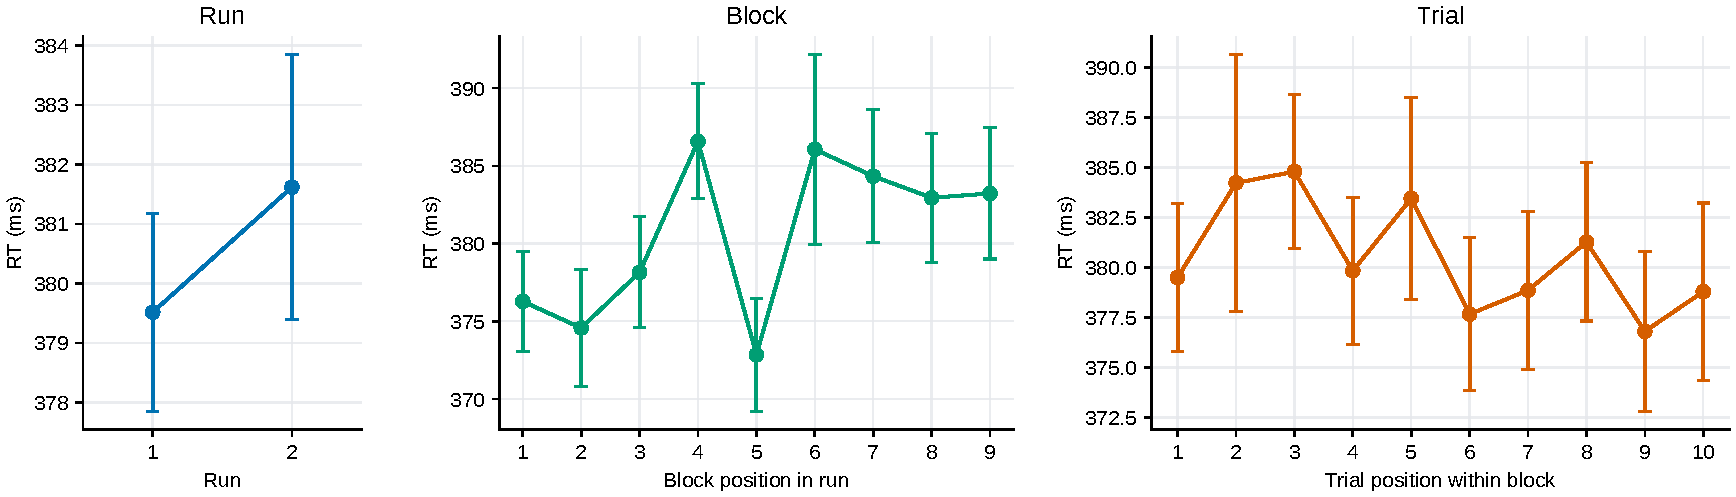
\includegraphics[width=\linewidth]{supplementary_figures/Sup_Figure28.pdf}
    \end{minipage}
    \caption{Supplementary behavioural reaction-time analyses. \textbf{A}, Trial-wise reaction-time distributions for OFF- and ON-medication sessions. \textbf{B}, Participant-level mean reaction times in the OFF- and ON-medication sessions. \textbf{C}, Mean reaction time across run, block position, and trial position within block, showing only modest temporal variation within the task.}
    \label{fig:RT_changes}
\end{figure}


Figure~\ref{fig:mixed_model} summarizes the main behavioural effects estimated from mixed-effects models of RT and RT variability. The trial-wise RT model included medication state, reward condition, their interaction, GVS condition and medication-by-GVS interactions, run, block position, trial position within run, and a random intercept for subject. 
\[
\begin{aligned}
\mathrm{RT}_{ms} \sim {} &
\mathrm{medication}_{on} \times \mathrm{reward}_{high}
+ \mathrm{medication}_{on} \times \mathrm{GVS}
+ \mathrm{run}
+ \mathrm{block\_position} \\
& + \mathrm{trial\_in\_run}
+ (1 \mid \mathrm{subject})
\end{aligned}
\]

RT variability was calculated as the root mean squared successive difference (RMSSD) between adjacent valid RTs within each subject, session, run, and GVS block, thereby avoiding transitions across stimulation blocks, rest periods, and run boundaries. The RT variability model included medication state, run, block position, high-reward fraction, GVS condition, and a random intercept for subject.
\[
\begin{aligned}
\mathrm{RT\_RMSSD}_{ms} \sim {} &
\mathrm{medication}_{on}
+ \mathrm{run}
+ \mathrm{block\_position}
+ \mathrm{reward\_high\_fraction} \\
& + \mathrm{GVS}
+ (1 \mid \mathrm{subject})
\end{aligned}
\]

The main observation is that medication ON significantly reduced RT relative to medication OFF, indicating faster responses under medication ($\beta = -26.37$ ms, 95\% CI $[-39.88, -12.86]$, $p < 0.001$). High reward also reduced RT ($\beta = -8.42$ ms, 95\% CI $[-14.50, -2.35]$, $p = 0.0066$), while the medication-by-reward interaction was not significant, suggesting that medication and reward effects were largely additive. Later block position was associated with slower RT ($\beta = 1.17$ ms per block, $p = 0.0059$). For GVS, the strongest mean-RT effect was observed for GVS7 relative to sham during medication OFF ($\beta = -18.21$ ms, $p = 0.0055$), but positive medication-by-GVS interactions indicated that this speeding effect was reduced or reversed during medication ON. For RT variability, medication and GVS condition did not show reliable effects, whereas run 2 and later block positions were associated with increased RT RMSSD. Overall, the figure suggests robust behavioural speeding by medication and high reward, weaker and medication-dependent GVS effects on mean RT, and a temporal increase in response variability across the task that likely reflects fatigue, instability, or changing engagement over time.

\begin{figure}[h]
    \centering
    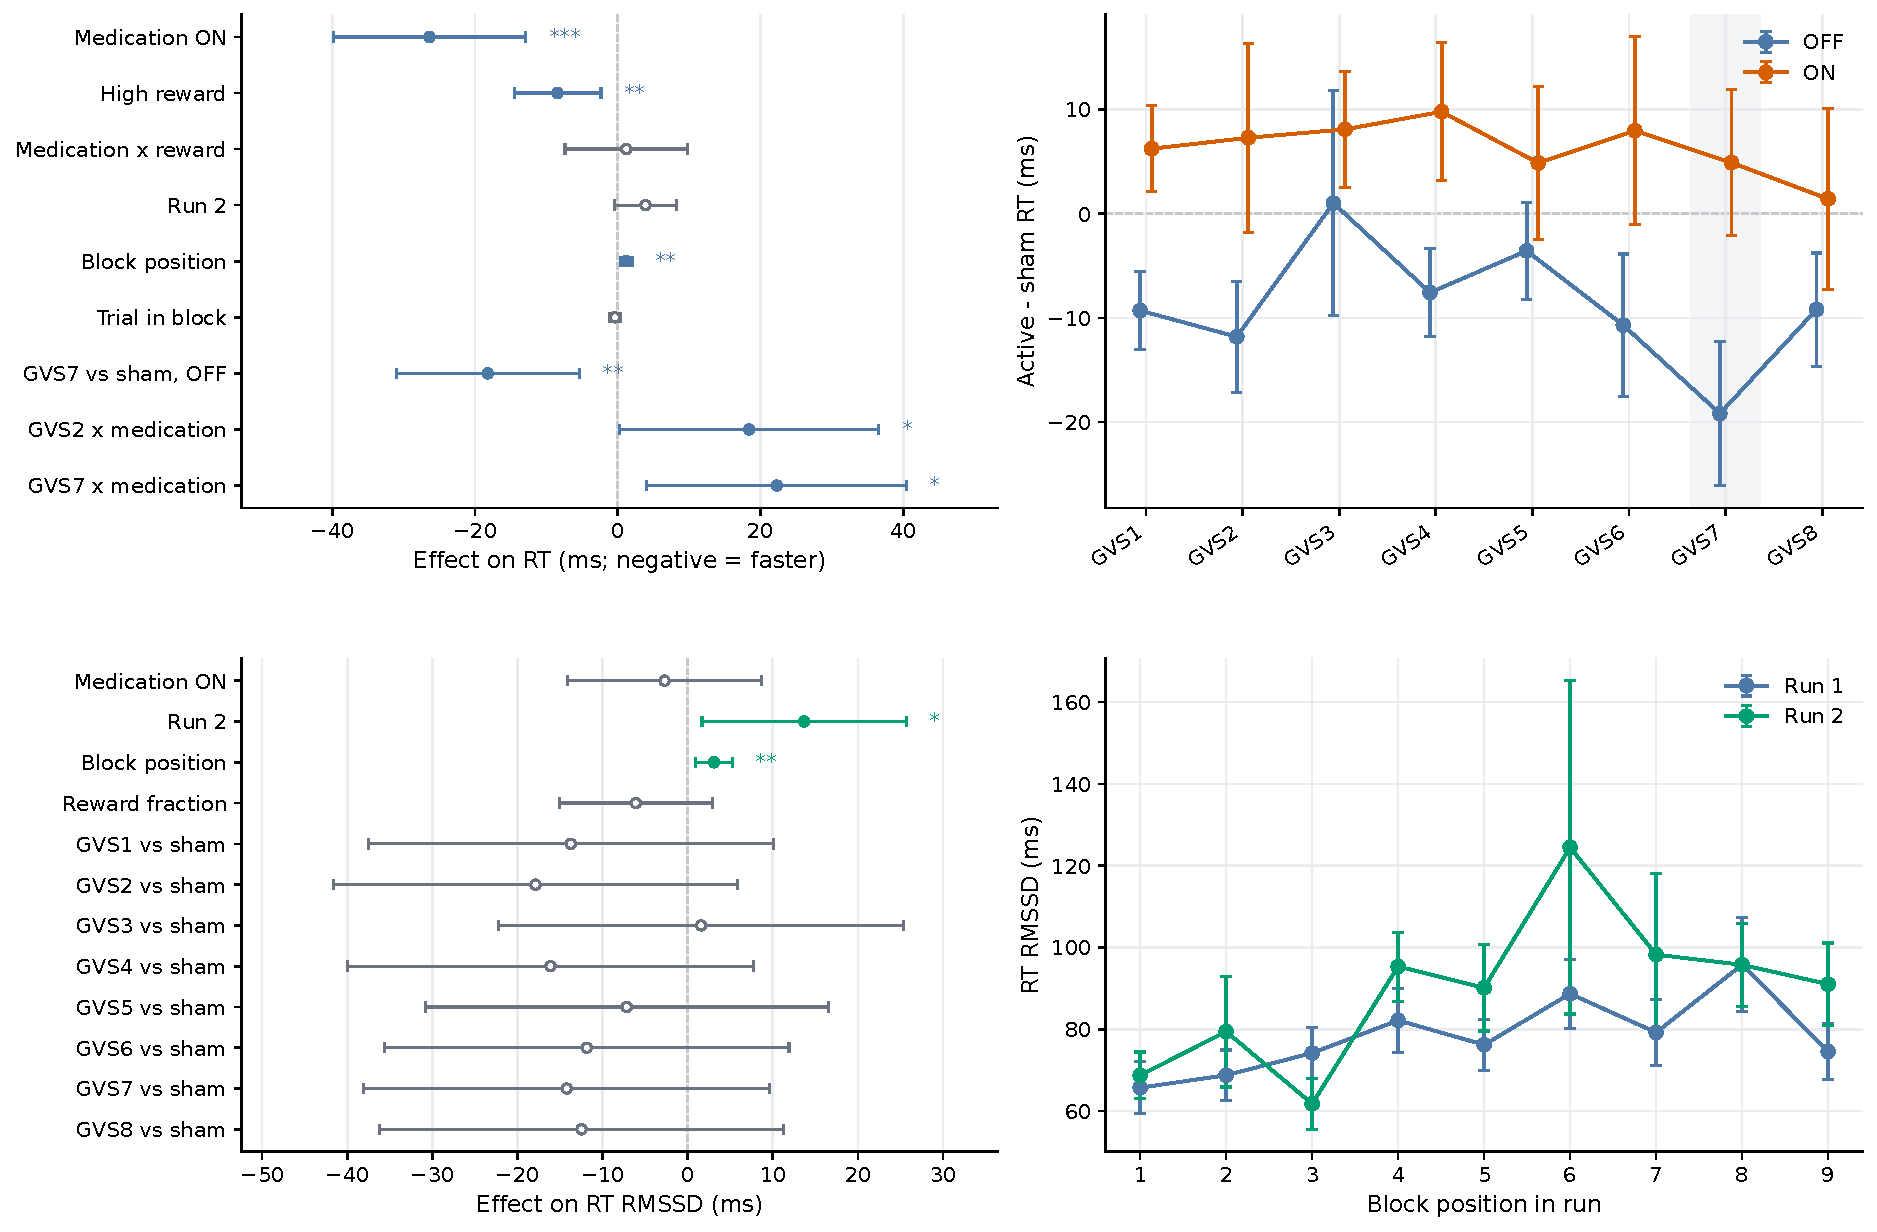
\includegraphics[width=\linewidth]{supplementary_figures/Sup_Figure29.pdf}
    \caption{Mixed-model behavioural effects on reaction time and RT variability. Upper left: fixed-effect estimates from a subject-random-intercept mixed model of valid trial-wise RT. Negative coefficients indicate faster responses. Upper right: active GVS minus sham RT differences, shown separately for medication OFF and ON sessions. Lower left: fixed-effect estimates from a subject-random-intercept mixed model of within-block RT variability, defined as RT RMSSD. Lower right: descriptive mean RT RMSSD by block position in run. Coefficient plots show model estimates with $95\%$ confidence intervals; filled colored markers and stars indicate nominally significant model terms (*$p \leq 0.05$, **$p \leq 0.01$, ***$p \leq 0.001$). Descriptive panels show mean $\pm$ SEM.}
    \label{fig:mixed_model}
\end{figure}


%###########################################################################################
\section{Participants information}

\begin{table}[h]
\centering
\caption{Clinical motor severity by medication state. MDS-UPDRS Part III ratings were available for all 18 participants. Values are reported as mean $\pm$ SD, median [range], or n/N.}
\label{tab:updrs_summary}

\renewcommand{\arraystretch}{1.3} % increase row spacing

\begin{tabular}{lccc}
\toprule
Measure & OFF medication & ON medication & ON--OFF \\
\midrule
MDS-UPDRS Part III total, mean $\pm$ SD 
& $37.3 \pm 17.3$ & $28.0 \pm 15.0$ & $-9.3 \pm 4.2$ \\

MDS-UPDRS Part III total, median [range] 
& $35.0$ [$10$, $75$] & $22.0$ [$7$, $61$] & $-9.0$ [$-17$, $-3$] \\

Improvement from OFF, \%, mean $\pm$ SD 
& -- & $26.6 \pm 9.1$ & -- \\

Minutes since last dose, median [range] 
& $931.5$ [$720$, $3006$] & $71.0$ [$36$, $102$] & -- \\

H\&Y stage, median [range] 
& $2$ [$1$, $4$] & $2$ [$0$, $3$] & -- \\

Dyskinesias present, n/N 
& $1/18$ & $3/18$ & -- \\

Dyskinesias interfered with ratings, n/N 
& $1/18$ & $0/18$ & -- \\
\bottomrule
\end{tabular}
\end{table}

\begin{table}[h]
\centering
\caption{MDS-UPDRS Part III domain scores by medication state. Domain groupings are descriptive and are defined by the item numbers listed in the table. Values are reported as mean $\pm$ SD.}
\label{tab:updrs_domains}
\renewcommand{\arraystretch}{1.3} % increase row spacing
\begin{tabular}{llccc}
\toprule
Domain & Items included & OFF mean $\pm$ SD & ON mean $\pm$ SD & ON-OFF mean $\pm$ SD \\
\midrule
Axial/signs & 3.1, 3.2, 3.9--3.14 
& $8.4 \pm 4.6$ & $7.3 \pm 4.5$ & $-1.2 \pm 1.3$ \\

Rigidity & 3.3A--3.3E 
& $6.5 \pm 3.9$ & $5.8 \pm 3.6$ & $-0.7 \pm 1.0$ \\

Limb bradykinesia & 3.4A--3.8B 
& $15.1 \pm 7.6$ & $11.3 \pm 7.8$ & $-3.8 \pm 3.3$ \\

Tremor & 3.15A--3.18 
& $7.2 \pm 5.3$ & $3.6 \pm 3.1$ & $-3.6 \pm 3.3$ \\
\bottomrule
\end{tabular}
\end{table}

%###########################################################################################
\section{GLM and GLMsingle analysis}
Spatial similarity between networks:

\begin{figure}[h]
    \centering
    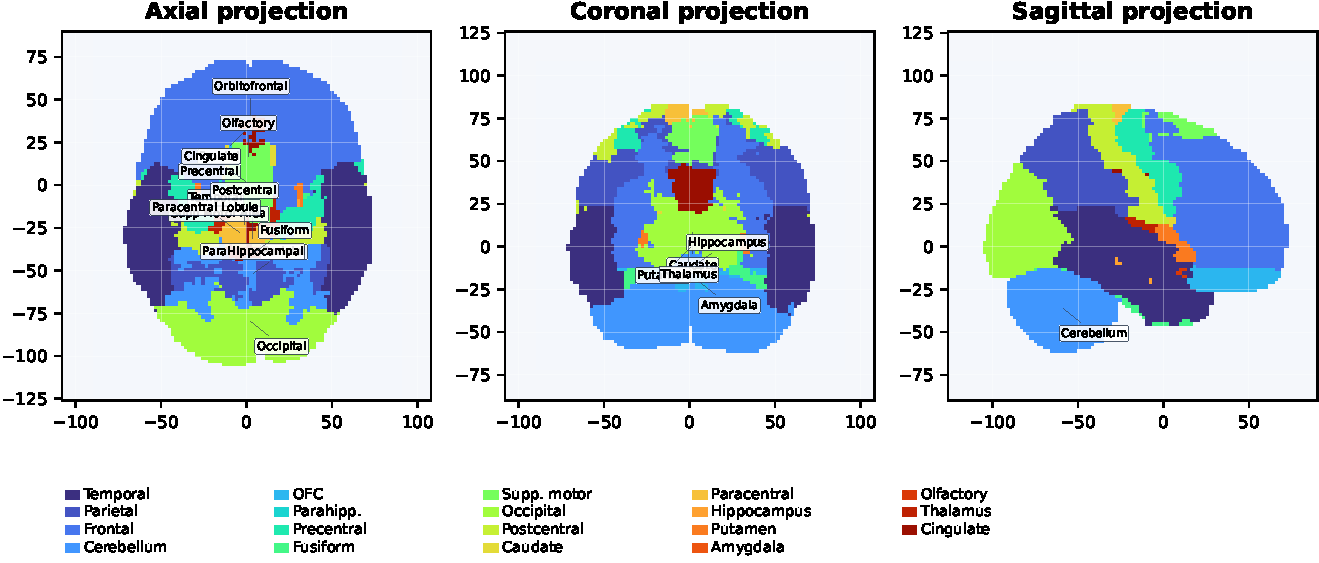
\includegraphics[width=0.4\linewidth]{supplementary_figures/Sup_Figure7.pdf}
    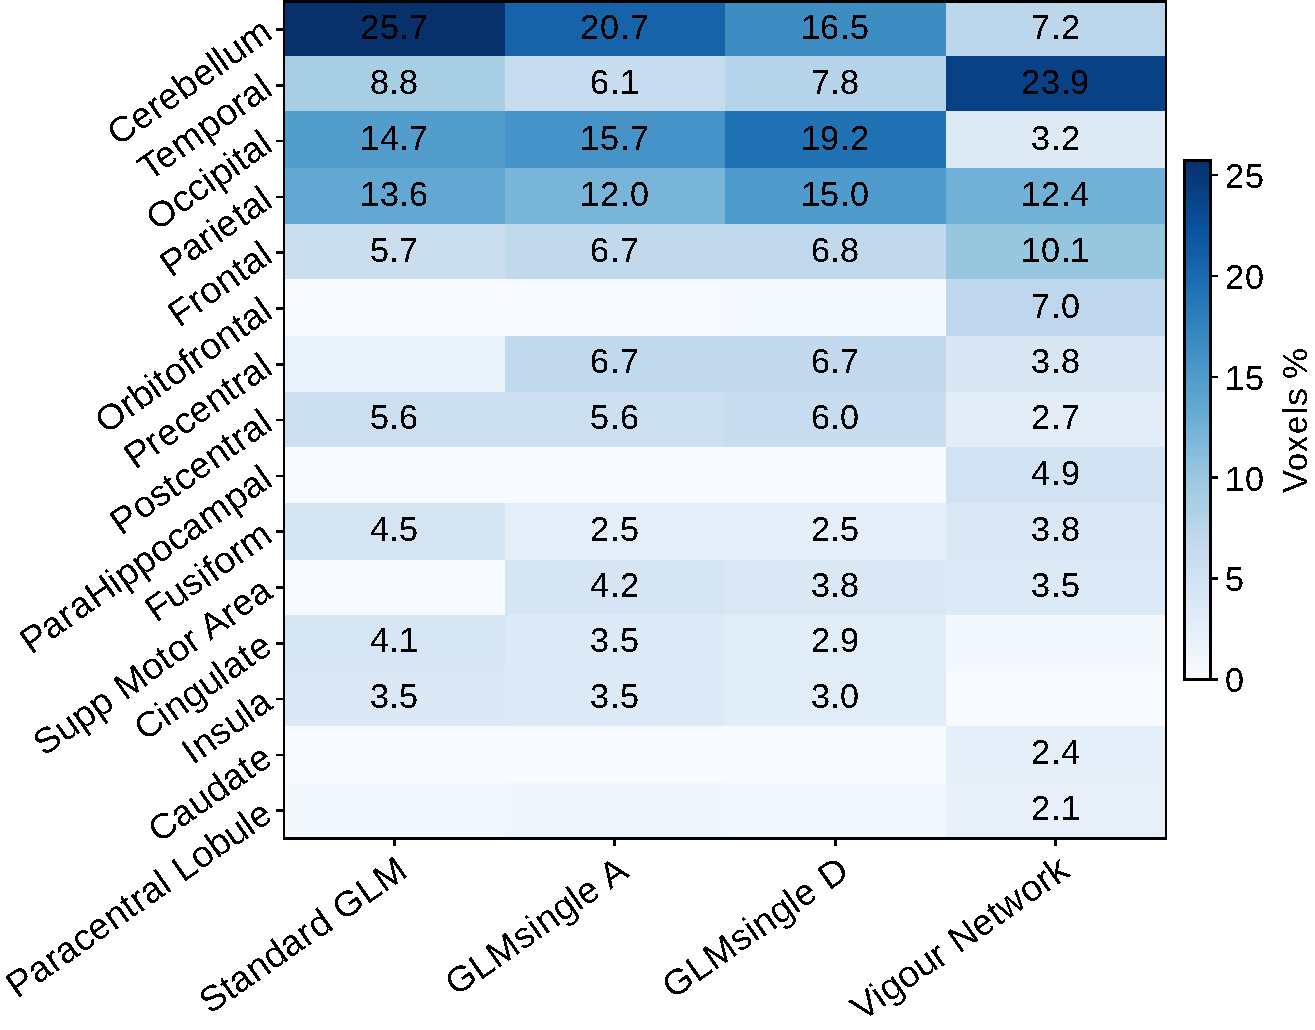
\includegraphics[width=0.5\linewidth]{supplementary_figures/Sup_Figure8.pdf}
    \caption{Caption}
    \label{fig:placeholder}
\end{figure}


%###########################################################################################
\section{Anatomical characterization of the vigour network}
\label{app:anatomy}

\subsection{ROI-wise composition of the final network}
I used this atlas to define ROIs in this study:

\begin{figure} [h]
    \centering
    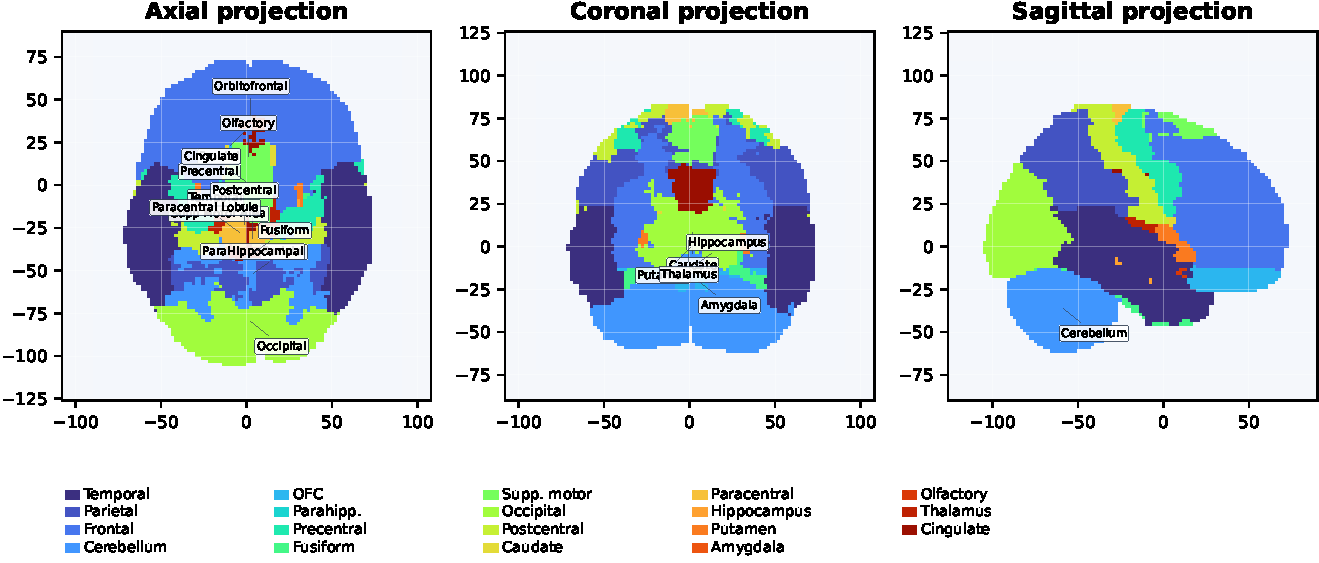
\includegraphics[width=\linewidth]{supplementary_figures/Sup_Figure4.pdf}
    \caption{Caption}
    \label{fig:placeholder}
\end{figure}

The vigour-network is marked by regions' function in the figure below:

\begin{figure}[h]
    \centering
    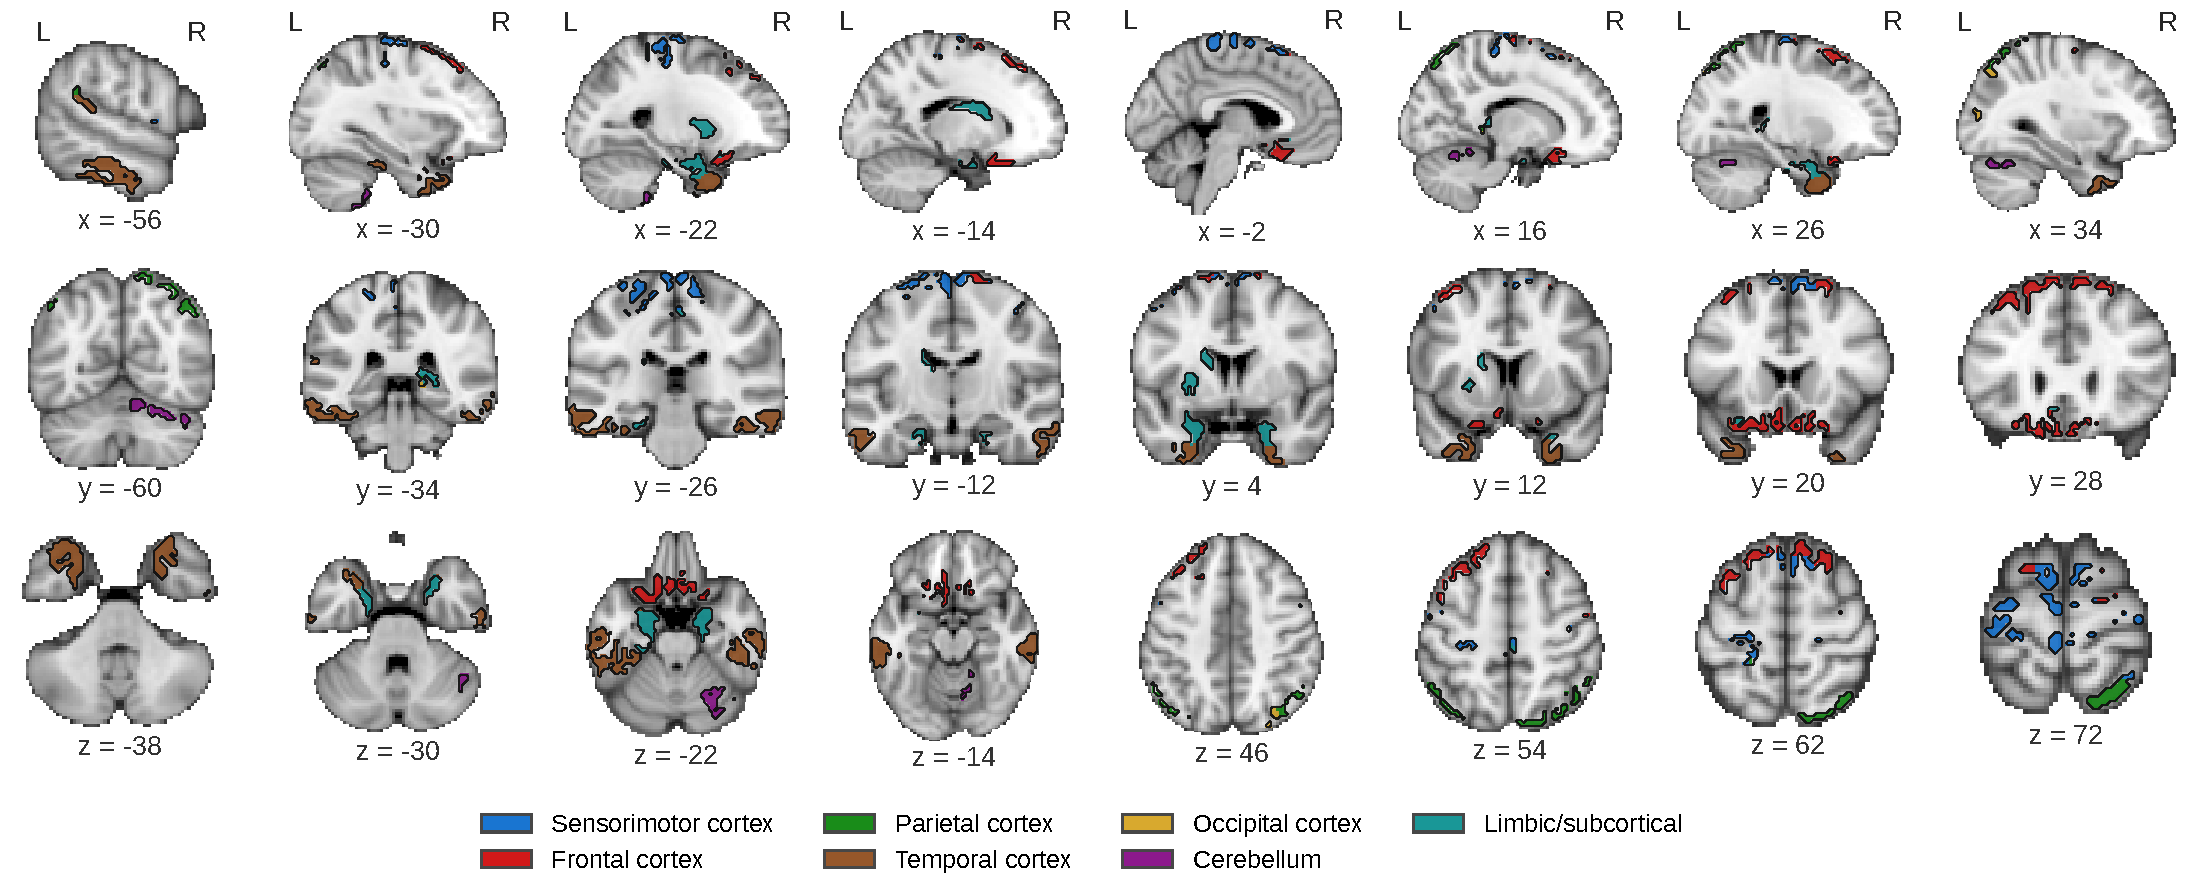
\includegraphics[width=\linewidth]{supplementary_figures/Sup_Figure5.pdf}
    \caption{Caption}
    \label{fig:placeholder}
\end{figure}

\begin{longtable}{@{} p{5.2cm} r r r r @{}}
\caption{ROI-wise composition of the suprathreshold vigour-related voxel-weight map shown in Fig.~\ref{fig:voxel_weights_task1}. ROIs are AAL3-derived bilateral anatomical groups and are ranked by their contribution to the selected map. The listed anatomical ROIs account for 97.03\% of selected voxels; the remaining 2.97\% fall outside the AAL3 labels used for this summary.\label{tab:roi_vigour_network}}\\
\toprule
ROI & ROI size & Selected voxels & \% ROI selected & \% of map \\
\midrule
\endfirsthead

\toprule
ROI & ROI size & Selected voxels & \% ROI selected & \% of map \\
\midrule
\endhead

\bottomrule
\endfoot

\bottomrule
\endlastfoot

Temporal cortex & 26584 & 1916 & 7.21 & 28.86 \\
Parietal cortex & 21027 & 685 & 3.26 & 10.32 \\
Frontal cortex & 34869 & 638 & 1.83 & 9.61 \\
Orbitofrontal cortex & 5372 & 518 & 9.64 & 7.80 \\
Cerebellum & 24414 & 489 & 2.00 & 7.37 \\
Parahippocampal gyrus & 2110 & 406 & 19.24 & 6.12 \\
Fusiform gyrus & 4827 & 291 & 6.03 & 4.38 \\
Supplementary motor area & 4518 & 286 & 6.33 & 4.31 \\
Precentral gyrus & 6907 & 252 & 3.65 & 3.80 \\
Caudate & 1666 & 163 & 9.78 & 2.46 \\
Occipital cortex & 21531 & 157 & 0.73 & 2.37 \\
Paracentral lobule & 2185 & 153 & 7.00 & 2.30 \\
Hippocampus & 1878 & 122 & 6.50 & 1.84 \\
Putamen & 2061 & 112 & 5.43 & 1.69 \\
Amygdala & 468 & 88 & 18.80 & 1.33 \\
Postcentral gyrus & 7715 & 72 & 0.93 & 1.08 \\
Olfactory cortex & 579 & 42 & 7.25 & 0.63 \\
Cingulate cortex & 7655 & 22 & 0.29 & 0.33 \\
Insular cortex & 3628 & 13 & 0.36 & 0.20 \\
Thalamus & 2213 & 11 & 0.50 & 0.17 \\
Rolandic operculum & 2319 & 3 & 0.13 & 0.05 \\
Pallidum & 573 & 2 & 0.35 & 0.03 \\
\end{longtable}

After normalizing by ROI size, the strongest selection is concentrated in temporal-limbic and striatal regions, particularly the parahippocampal gyrus, amygdala, caudate, orbitofrontal cortex, and temporal cortex. Motor-related regions are also represented, including the supplementary motor area, paracentral lobule, precentral gyrus, parietal cortex, and cerebellum, but they do not dominate the ROI-normalized profile. Thus, the map contains a motor-related component, but its strongest ROI-level enrichment is distributed across temporal-limbic and associative regions rather than being confined to primary motor cortex.

\subsection{Comparison with the task-engagement reference map}
The tables below provide a compact summary of the limited overlap between the final vigour-related network and the task-engagement reference map, including both global overlap metrics and region-wise voxel counts.

\begin{table}[h]
\centering
\caption{Comparison of the full-constraint vigour network and the task-activation reference map.\label{tab:two_networks}}
\small
\begin{threeparttable}

\begin{tabularx}{\textwidth}{
    >{\raggedright\arraybackslash}p{3.1cm}
    >{\centering\arraybackslash}p{1.6cm}
    >{\centering\arraybackslash}p{2.8cm}
    >{\raggedright\arraybackslash}X
}
\toprule
\textbf{Network} & \textbf{Voxel count} & \textbf{Shared voxels (\% of network)} & \textbf{Main anatomical labels} \\
\midrule
Task-activation map & 21,610 & 503 (2.33\%) &
Cerebellum/vermis and thalamic nuclei; supramarginal cortex; occipital, parietal, and insular cortex \\

Full-constraint vigour network & 5,957 & 503 (8.44\%) &
Parahippocampal cortex; amygdala; middle temporal pole; inferior temporal cortex; rectus and medial/posterior orbitofrontal cortex \\
\bottomrule
\end{tabularx}

\begin{tablenotes}[flushleft]
\footnotesize
\item ROI metrics: same-voxel overlap $=503$ voxels; Dice coefficient $=0.036$; Jaccard index $=0.019$.
\item The shared voxels were concentrated most in putamen, cerebellar lobules 6/8, middle occipital cortex, paracentral lobule, superior parietal cortex, and postcentral gyrus.
\item In the GLM/GLMsingle comparison, the vigour network showed low overlap with each activation map: Dice $=0.09$ with standard GLM, $0.11$ with GLMsingle A, and $0.10$ with GLMsingle D.
\end{tablenotes}
\end{threeparttable}
\end{table}

\begin{table}[htbp]
\centering
\scriptsize
\caption{ROI-level voxel overlap between the full model and task-only activation network.}
\label{tab:ablation_full_vs_task_only_roi}

\begin{tabularx}{\textwidth}{@{}lccc>{\raggedright\arraybackslash}X@{}}
\toprule
ROI &
\makecell{Shared voxel\\n (\% ROI)} &
\makecell{Vigour network\\n (\% ROI)} &
\makecell{Task activation\\network n (\% ROI)} &
Voxel-level relation \\
\midrule
Putamen & 90 (6.03\%) & 22 (1.47\%) & 620 (41.55\%) & Shared voxels present \\
Pallidum & 0 (0.00\%) & 2 (0.38\%) & 171 (32.70\%) & Both maps in ROI, no shared voxels \\
Fusiform & 9 (0.20\%) & 294 (6.62\%) & 970 (21.83\%) & Shared voxels present \\
Parietal & 51 (0.28\%) & 607 (3.37\%) & 4,301 (23.87\%) & Shared voxels present \\
Insula & 0 (0.00\%) & 13 (0.37\%) & 908 (25.73\%) & Both maps in ROI, no shared voxels \\
Postcentral & 20 (0.29\%) & 50 (0.73\%) & 1,659 (24.16\%) & Shared voxels present \\
ParaHippocampal & 0 (0.00\%) & 278 (20.87\%) & 5 (0.38\%) & Both maps in ROI, no shared voxels \\
Amygdala & 0 (0.00\%) & 86 (20.92\%) & 0 (0.00\%) & Vigour network only in ROI \\
Occipital & 64 (0.35\%) & 89 (0.49\%) & 3,474 (19.14\%) & Shared voxels present \\
Cerebellum & 225 (0.98\%) & 250 (1.09\%) & 4,034 (17.65\%) & Shared voxels present \\
Temporal & 8 (0.03\%) & 1,769 (7.43\%) & 2,007 (8.43\%) & Shared voxels present \\
Paracentral\_Lobule & 19 (1.18\%) & 127 (7.86\%) & 103 (6.37\%) & Shared voxels present \\
Cingulate & 0 (0.00\%) & 20 (0.35\%) & 724 (12.77\%) & Both maps in ROI, no shared voxels \\
Rolandic\_Oper & 0 (0.00\%) & 3 (0.16\%) & 239 (12.63\%) & Both maps in ROI, no shared voxels \\
Precentral & 15 (0.27\%) & 225 (3.99\%) & 420 (7.46\%) & Shared voxels present \\
Orbitofrontal & 0 (0.00\%) & 466 (9.94\%) & 15 (0.32\%) & Both maps in ROI, no shared voxels \\
Caudate & 0 (0.00\%) & 121 (10.04\%) & 0 (0.00\%) & Vigour network only in ROI \\
Supp\_Motor\_Area & 2 (0.06\%) & 282 (8.31\%) & 41 (1.21\%) & Shared voxels present \\
Thalamus & 0 (0.00\%) & 9 (1.22\%) & 57 (7.70\%) & Both maps in ROI, no shared voxels \\
Hippocampus & 0 (0.00\%) & 66 (6.07\%) & 29 (2.67\%) & Both maps in ROI, no shared voxels \\
Olfactory & 0 (0.00\%) & 36 (7.83\%) & 0 (0.00\%) & Vigour network only in ROI \\
Frontal & 0 (0.00\%) & 632 (2.15\%) & 1,258 (4.29\%) & Both maps in ROI, no shared voxels \\
Cerebral\_Cortex & 0 (0.00\%) & 7 (0.20\%) & 72 (2.04\%) & Both maps in ROI, no shared voxels \\
\bottomrule
\end{tabularx}
\end{table}

%###########################################################################################
\section{Medication-state analyses}
\subsection{Control analysis: no evidence for preferential ON-state stabilization}



%###########################################################################################
\section{GVS-related analyses}
\label{app:gvs}


\end{document}